\section{Morfogénesis}

Mordvintsev et al. en \cite{mordvintsevNCA} diseñaron un autómata celular neuronal que permite a una célula crecer para formar un patrón, persistir en el tiempo, regenerarse e incluso rotar. Diseñaron un modelo que utiliza un autómata celular continuo con un vector de estados de 16 dimensiones. Este modelo incorpora gradientes espaciales utilizando filtros de Sobel. 

\begin{figure}[htbp]
	
	\centering
	
	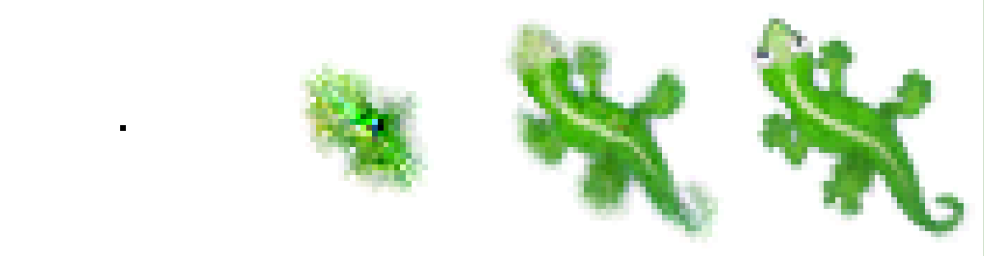
\includegraphics[width=0.6\linewidth]{img/morfogenesis.png}
	
	\caption{Evolución del \textit{emoji} de una lagartija a partir de una única célula activa después de 219 pasos evolutivos \cite{mordvintsevNCA}.}
	
	\label{fig:morfogenesis}
	
\end{figure}

El autómata celular neuronal diseñado tiene las siguientes características (las cuales fueron retomadas por múltiples autores que tomaron a \cite{mordvintsevNCA} como referencia):

\begin{itemize}
	
	\item El vector de cada célula (cada valor en un rango de $[0,1]$) incluye los canales RGB y un canal $\alpha$ que funciona como umbral para definir si una célula está viva o muerta (establece el resto de valores del vector a $0$ si $\alpha \leq 0.1$). 
	
	
	
	Considerando las dimensiones $(\text{largo}, \text{ancho}, 16)$ y un kernel de $3 \times 3$, se calcula el gradiente en las dos direcciones ($x$ y $y$) usando un filtro Sobel. Esto genera un nuevo vector que se utilizará como entrada para la red neuronal.
	
	\[ 
	16 (\text{estado propio}) + 16 (\text{gradiente en } x) + 16 (\text{gradiente en } y) = 48 
	\]
	
	
	
	\item Se usaron convoluciones de $1 \times 1$ con una función \textit{ReLU} y alrededor de $8000$ parámetros entrenables y devuelve un $\delta$ que se suma al estado actual de célula antes del siguiente paso. 
	
	
	
	\item Se omite el cálculo para las células muertas y la actualización de cada célula se realiza con una probabilidad del $50\%$. La actualización debe ser estocástica para lograr un mejor rendimiento \cite{NiklassonNCA}. 
	
\end{itemize}

Eyvind Niklasson et al. \cite{NiklassonNCA} compararon el rendimiento del modelo en \cite{mordvintsevNCA} con actualización síncrona y asíncrona. Donde, tras haber llevado a cabo pruebas con diferentes tamaños de paso, concluyeron que la función de pérdida crece exponencialmente cuando la actualización es síncrona. Sin embargo, esto ocurre únicamente cuando el tamaño de paso es mayor a uno.

Una hipótesis de este comportamiento es que, al tener células que se actualizan en diferentes periodos de tiempo, cada célula puede conocer parte del contexto de su vecindad. Esto no se logra únicamente conociendo los valores actuales de cada vecino.

Se realizaron los siguientes experimentos en \cite{mordvintsevNCA}:

\begin{enumerate}
	
	\item Crecer una única célula activa para formar una figura dada mediante \textit{backpropagation}. Cuando el autómata celular llega a la figura deseada, si se siguen aplicando las reglas de evolución, puede crecer sin límites, quedarse en la misma figura, eliminar todas las células o crear patrones que son caóticos o que se repiten.
	
	
	
	\item Convertir las figuras objetivo en atractores usando \textit{sample pool}. Se entrenó mediante múltiples condiciones iniciales, obtenidas a partir de entrenamientos fallidos, para llegar al objetivo desde diferentes configuraciones. 
	
	
	
	\item Regenerar partes de la figura. Se eliminaron partes de la figura objetivo y se añadieron al conjunto de entrenamiento.
	
	
	
	\item Rotaron la figura objetivo. Dado que los filtros de Sobel funcionan como direcciones ortogonales, se puede aplicar una rotación mediante: 
	
	\[ \begin{bmatrix}
		
		K_x & K_y
		
	\end{bmatrix} = \begin{bmatrix}
		
		cos \theta & -sin \theta \\
		
		sin \theta & cos \theta
		
	\end{bmatrix} \cdot \begin{bmatrix}
		
		Sobel_x & Sobel_y
		
	\end{bmatrix} \]
	
	Para modificar el ángulo sin necesidad de reentrenar el modelo.
	
\end{enumerate}

\subsection{Autómatas celulares neuronales isotrópicos}

En \cite{IsoNCA}, \cite{IsoNCA2} y \cite{SteerableNCA}, Mordvintsev et al. presentan una nueva configuración que no tenga una dirección preferida, la cual nombraron autómatas celulares neuronales isotrópicos.

Para que esta regla sea isotrópica, es necesario que sea independiente de la dirección (sin distinguir ``arriba'' de ``izquierda''). Esto permite crear rotaciones o simetrías sin que el sistema se descontrole.

Se sustituyen las funciones de los filtros de Sobel en \cite{mordvintsevNCA} por un único filtro laplaciano:

\[
K_{lap} = \begin{bmatrix}
	
	1 & 2 & 1 \\
	
	2 & -12 & 2 \\
	
	1 & 2 & 1 
	
\end{bmatrix}
\]

El cual se concatena al vector de cada célula y alimenta a una red neuronal artificial de $9408$ parámetros. 

A continuación, se describen los resultados obtenidos con dos diferentes enfoques:

\begin{enumerate}
	
	\item Estrategia de \textit{seed} (semilla) estructurada: Se necesitan al menos tres células con valores diferentes y no colineales para definir la orientación y la posición. Modificar la posición de estos puntos implica una evolución acorde a la posición de los mismos.
	
	\item Estrategia de una única \textit{seed}: Se modifica la función de pérdida para que sea invariante ante rotaciones y reflejos. Para evitar comparar la figura resultante con todas las rotaciones posibles, se mapean ambas figuras a coordenadas polares y, para cada posible ángulo de rotación, se calcula la diferencia. Para disminuir la complejidad computacional, se aplica la transformada rápida de Fourier y se hace uso del teorema de la convolución:
	
	\[
	s * t = \mathcal{F}^{-1} (\mathcal{F}(S) \cdot \mathcal{F}(T)) 
	\]
	
	Se obtienen todas las diferencias únicamente como una multiplicación de transformadas.
	
	
	
	Para evitar que se formen patrones simétricos mezclados (como figuras con cabeza-cabeza o cola-cola), se agrega un nuevo canal llamado \textit{binary auxiliar channel} que da valores de $-0.5$ y $0.5$ a la parte superior e inferior de la imagen.
	
	
	
	Con estas nuevas configuraciones se puede obtener el mismo resultado que en \cite{mordvintsevNCA}, pero sin la dependencia de una dirección explícita y con una red neuronal artificial con menos parámetros.
	
\end{enumerate}

\subsection{Autoclasificación}

Mordvintsev et al. en \cite{MNIST} utilizan los autómatas celulares neuronales para la autoclasificación de MNIST\footnote{Conjunto de datos de imágenes $28 \times 28$ de números en el rango $[0,9]$} las cuales fueron binarizadas con un umbral de $0.1$. 

El objetivo es que, a partir de una configuración inicial de células vivas, el sistema pueda reconocer la forma solo usando reglas locales. En este caso, se trata de identificar los números de MNIST.

Estos son los cambios del autómata celular \textit{MNIST CA} respecto al modelo original \cite{mordvintsevNCA}:

\begin{itemize}
	
	\item Vector de la célula: Originalmente se usaban los canales RGB; ahora se usan 10 canales que funcionan como distribución de probabilidad de cada posible número. Durante la evaluación se utiliza el mayor de ellos.
	
	
	
	\item Célula viva o muerta: En \cite{mordvintsevNCA} se define mediante el canal $\alpha$, pero las células muertas siguen siendo visibles para el resto. En \cite{MNIST}  únicamente interactúan las células vivas.
	
	
	
	\item Topología: Todas las células son un único componente conexo.
	
\end{itemize}

Con el nuevo modelo, Mordvintsev et al. pudieron realizar clasificaciones con una precisión del $95.3\%$ con una función de pérdida $L_2$ y ruido añadido. Este experimento demostró que los autómatas celulares neuronales no solo pueden generar patrones y autorregenerarse, sino también realizar tareas de clasificación distribuidas sin una capa de decisión global.

Aunque los modelos \textit{Growing CA} y \textit{MNIST CA} son robustos frente a diferentes tipos de perturbaciones, su comportamiento se puede ver afectado por estados individuales de las células, parámetros del modelo y el campo perceptivo (la manera en cómo las células perciben su vecindad).

Es por esto que Randazzo et al. \cite{randazzoNCA} buscan enfrentar estrategias adversarias en el mismo espacio celular para estudiar la reprogramación de los autómatas celulares mediante dos experimentos:

\begin{enumerate}
	
	\item Inyección de adversarios: Se entrena un nuevo modelo de autómata celular, que se coloca en el entorno que ejecuta uno de los modelos originales, para secuestrar el comportamiento del colectivo.
	
	
	
	\item Perturbación de estados: A un modelo ya entrenado, se le aplican perturbaciones a todas las células del sistema de forma simultánea.
	
\end{enumerate}

Para la inyección de adversarios se utilizan dos modelos: el modelo original \textit{MNIST CA} con probabilidad de $90\%$ y un nuevo modelo que clasifica a todos los números como ``ocho'' ($10\%$).  Se introducen varias células invasoras en figuras que ya han sido clasificadas, y estas células muestran un comportamiento dominante al clasificar todos los elementos como "ocho". Además, una vez retiradas las células invasoras, el sistema es capaz de recuperarse la mayoría de las veces.

Sin embargo, al aplicar el mismo procedimiento para \textit{Growing CA}, los resultados no tuvieron el mismo rendimiento. Probaron modificar la morfología de la imagen de una lagartija sin cola y con otro color, pero ninguna estrategia fue capaz de invadir por completo el modelo original. 

Una hipótesis es que \textit{MNIST CA} no necesita cambiar completamente su valor para producir algo diferente de lo que generaba antes, ya que el estado de la mutación es un estado que el modelo original ya tenía en cuenta. Por otro lado, al cambiar el color y la forma en \textit{Growing CA}, se están explorando configuraciones nunca antes vistas por el modelo original.

Para el segundo experimento (perturbación de estados), se sigue la línea de modificar el color y la forma de la imagen de una lagartija. Se aplica una perturbación global de estados cada paso de tiempo con el objetivo de identificar la perturbación específica que dé como resultado un patrón estable.

En cada paso evolutivo se multiplica el vector de cada célula por una matriz simétrica $A$ de $16 \times 16$ \cite{mordvintsevNCA}. Para definir los valores de la matriz, se inicia con una matriz simétrica $I$ y, a diferencia de \textit{Growing CA}, la configuración inicial se establece como la figura objetivo del modelo original.

Esta configuración permite crecer un sistema con perturbaciones, alterar su forma y color una vez crecido y modificar el impacto y el número de perturbaciones posibles. Al manejar matrices simétricas, se puede representar como 

\[A = Q \Lambda Q^T\] 

donde: 

\begin{itemize}
	
	\item $\Lambda$ es la matriz diagonal de los valores propios.
	
	\item $Q$ es la matriz unitaria de los vectores propios.
	
\end{itemize} 

Si $\Lambda = I \to A = I$, por lo que no existe perturbación (multiplicación por matriz identidad). Bajo esta premisa, se propone la siguiente fórmula:

\[ A_k = Q(kD + I)Q^T\]

Donde:

\begin{itemize}
	
	\item $A$ es la matriz original.
	
	\item $k$ es el factor de escala.
	
	\item $D$ es la dirección de la perturbación $\Lambda - I$ en el espacio de valores propios. 
	
\end{itemize}

Si $k = 0$, no existe perturbación en el sistema:

\begin{gather*}
	A_k = Q(0D + I)Q^T \\
	A_k = Q I Q^T
\end{gather*}

Si $k = 1$, se conserva la perturbación original:

\begin{gather*}
	A_k = Q(1D + I)Q^T \\
	A_k = Q(\Lambda - I + I)Q^T \\
	A_k = Q \Lambda Q^T
\end{gather*}

Mostrando que se puede escalar el tamaño de la perturbación, incluso con perturbaciones inversas con $k = -1$.

Si consideramos dos perturbaciones cuyos vectores propios son similares: $A_k = Q(k_AD_A + I)Q^T$ y $B_k = Q(k_B D_B + I)Q^T$, podemos combinarlos como

\[ comb(A_k, B_k) = Q (k_A D_A + k_B D_B + I) Q^T = k_A A + k_B B + (1 - k_A - k_B) I \]

Esta nueva combinación permite configurar múltiples perturbaciones, las cuales se vuelven más sensibles conforme aumentan los $k$.

Estos experimentos muestran cómo los autómatas celulares neuronales pueden ser vulnerables a diferentes estrategias y cómo las mutaciones ``exactas'' pueden modificar la estructura de todo el sistema, mostrando un comportamiento similar a lo que ocurre en teoría de juegos evolutivos.

Todas estas representaciones han tenido un lugar en un espacio bidimensional (2D). A continuación se presentan algunas propuestas en espacios tridimensionales (3D). 

\subsection{Representaciones tridimensionales}

Zhang et al. \cite{GCA} proponen un modelo generativo tridimensional denominado autómata celular generativo que extiende el paradigma de los autómatas celulares hacia la generación progresiva de formas 3D. A diferencia de enfoques que intentan reconstruir directamente la forma completa, autómata celular generativo formula el proceso como una cadena de Markov, donde cada paso corresponde a una transición local sobre una rejilla tridimensional. 

El modelo se entrena para que estas reglas locales, al repetirse, converjan hacia formas específicas. Para ello, se representa la forma como puntos de superficie en una rejilla 3D y se emplea una red convolucional dispersa que opera únicamente sobre las regiones activas.

Durante el entrenamiento, se utilizan secuencias ligeramente distintas a las cadenas de muestreo reales, pero que convergen hacia las formas del conjunto de datos. Esto permite que el modelo aprenda reglas de transición robustas, capaces de generar formas diversas desde configuraciones parciales. Con una sola inferencia, el sistema puede tomar diferentes ejemplos de la distribución que ha aprendido, obteniendo buenos resultados en tareas de completar y generar formas en 3D.

Este enfoque es una aportación importante a la morfogénesis computacional, ya que muestra que las reglas locales que se autoorganizan pueden aplicarse a estructuras 3D complejas utilizando redes neuronales adaptadas.

En \cite{GCA}, se muestra que la autoorganización local se puede escalar a tres dimensiones. Por otro lado, Shyam Sudhakaran y otros \cite{NCA3D} amplían el trabajo de \cite{mordvintsevNCA} a tres dimensiones, usando el juego de Minecraft como espacio celular\footnote{En Minecraft, se pueden crear estructuras estáticas (como árboles) y estructuras dinámicas (como máquinas voladoras)}. El autómata celular neuronal entrenado puede crear estructuras de hasta 3584 bloques utilizando 50 bloques diferentes, manteniendo las propiedades de regeneración de su versión en 2D.

Una entidad en Minecraft se representa como una red 3D donde cada elemento es un vector que almacena (1) el tipo de bloque (incrustado en un vector \textit{one-hot}), (2) su estatus (replicando el comportamiento del canal $\alpha$ de \cite{mordvintsevNCA}) y (3) estados ocultos.

Se utilizan convoluciones para permitir la generación y manipulación de estructuras 3D. Además, se sustituye el uso de filtros de Sobel por una red de percepción aprendible con un kernel de $3 \times 3 \times 3$, \textit{stride}\footnote{Cuántas posiciones se desplaza el \textit{kernel} sobre la entrada en cada operación de convolución} de 1 y canales de salida equivalentes a tres veces el número de canales del estado celular. Esta red permite que el sistema aprenda activamente a percibir su entorno local, adaptando sus filtros durante el entrenamiento y capturando patrones espaciales relevantes de manera dinámica.

Se utiliza una actualización estocástica y un umbral de activación similar a \cite{mordvintsevNCA}. Finalmente, todos los modelos se inicializan con una distribución normal estándar, con media cero y desviación estándar en el rango de $0.0001$ a $0.1$, lo que proporciona un punto de partida estable para el entrenamiento y la evolución del sistema. Este sistema hereda las propiedades regenerativas de su versión 2D.

Finalmente, Horibe et al. \cite{horibe} lleva las propiedades regenerativas al mundo físico. Se implementa el enfoque regenerativo en robots blandos mediante autómata celular neuronal. Cada robot tiene un conjunto de volúmenes de reposo para cada vóxel\footnote{Unidad básica de un espacio tridimensional, similar a un píxel en imágenes 2D, pero con volumen}. Estos volúmenes se activan con una señal global que tiene forma de onda sinusoidal, lo que causa que se expandan y se contraigan. Esta dinámica permite simular locomoción a través de ciclos de actuación, evaluando el desplazamiento del centro de masa como métrica de fitness. Los robots blandos se componen de distintos tipos de vóxeles: músculos en fase y contrafase, huesos rígidos y flexibles, cada uno con un rol en la locomoción.

El modelo entrenado demuestra que los robots blandos pueden recuperar parcialmente su morfología original tras sufrir daño y restaurar su capacidad de movimiento sin intervención externa. Este comportamiento surge de la dinámica autoorganizada del autómata celular neuronal, que codifica de manera implícita la forma objetivo y su capacidad de reparación.

Para evaluar la capacidad de locomoción y regeneración de los robots blandos generados mediante autómatas celulares neuronales, se emplea el simulador físico Voxelyze. Los experimentos se realizan en configuraciones 2D y 3D, utilizando rejillas de $7 \times 7$ y $9 \times 9 \times 9$ vóxeles, respectivamente. Las condiciones de frontera tipo Dirichlet limitan el crecimiento morfológico a regiones internas ($5 \times 5$ en 2D y $7 \times 7 \times 7$ en 3D).

Este entorno permite comprobar cómo los autómatas celulares neuronales se organizan por sí mismos para crear formas que son funcionales y resistentes. Además, proporciona una base cuantitativa para comparar la eficiencia locomotora antes y después de procesos de regeneración. La estructura en voxeles ayuda a combinar reglas locales y programación distribuida, y se relaciona con modelos inspirados en la biología sobre cómo se forma la estructura.

En conjunto, estos trabajos evidencian cómo los autómatas celulares neuronales pueden extender sus principios regenerativos y de autoorganización a dominios tridimensionales cada vez más complejos. Mientras Autómatas celulares generativos establece un marco generativo para formas 3D a partir de reglas locales aprendidas, los experimentos en Minecraft muestran que dichas propiedades pueden preservarse incluso en entornos con alta variabilidad estructural. Finalmente, la aplicación en robots blandos confirma el potencial bioinspirado de los autómatas celulares neuronales: no solo permiten generar morfologías funcionales, sino que además dotan a los sistemas físicos de resiliencia ante daños, abriendo camino hacia formas de robótica autorreparable.

Otra forma de implementar los autómatas celulares neuronales en 3D es mediante planos y texturas autoorganizadas que cubren la superficie de un objeto tridimensional. 